\section{Introduction}\label{introduction}

\begin{frame}{Good Quote}

\Large

\begin{quote}
``You must stick to your conviction, but be ready to abandon your
assumptions.''

--- Dennis Waitley
\end{quote}

\end{frame}

\begin{frame}{GLMs}

\large
Generalized Linear Models (GLMs):

\begin{enumerate}
\def\labelenumi{\arabic{enumi}.}
\tightlist
\item
  Are extensions of linear regression to areas where assumptions of
  normality and homoskedasticity do not hold
\item
  There are several versions of GLM's, each for different types and
  distributions of outcomes.
\end{enumerate}

We are going to go through several of the most common GLMs.

\end{frame}

\begin{frame}{Types}

\large 

We discuss:

\begin{enumerate}
\def\labelenumi{\arabic{enumi}.}
\tightlist
\item
  Logistic Regression
\item
  Poisson Regression
\item
  GLM with Gamma distribution
\item
  Negative binomial
\item
  Beta Regression
\end{enumerate}

\end{frame}

\section{Logistic Regression}\label{logistic-regression}

\begin{frame}{Logistic Regression}

\large
For binary outcomes (e.g., yes or no, correct or incorrect, sick or
healthy)

\[
logit(Y) = \beta_0 + \beta_1 X_1 + ... + \epsilon
\]

where \(logit(Y) = ln\Big(\frac{Prob(Y = 1)}{1 - Prob(Y = 1)}\Big)\)

\end{frame}

\begin{frame}[fragile]{Prep Data}

\small

\begin{Shaded}
\begin{Highlighting}[]
\NormalTok{## First creating binary depression variable}
\NormalTok{## Use mutate()}
\NormalTok{df <-}\StringTok{ }\NormalTok{df }\OperatorTok
\StringTok{  }\KeywordTok{mutate}\NormalTok{(}\DataTypeTok{dep =}\NormalTok{ dpq010 }\OperatorTok{+}\StringTok{ }\NormalTok{dpq020 }\OperatorTok{+}\StringTok{ }\NormalTok{dpq030 }\OperatorTok{+}\StringTok{ }\NormalTok{dpq040 }\OperatorTok{+}\StringTok{ }\NormalTok{dpq050 }\OperatorTok{+}
\StringTok{               }\NormalTok{dpq060 }\OperatorTok{+}\StringTok{ }\NormalTok{dpq070 }\OperatorTok{+}\StringTok{ }\NormalTok{dpq080 }\OperatorTok{+}\StringTok{ }\NormalTok{dpq090) }\OperatorTok
\StringTok{  }\KeywordTok{mutate}\NormalTok{(}\DataTypeTok{dep2 =} \KeywordTok{ifelse}\NormalTok{(dep }\OperatorTok{>=}\StringTok{ }\DecValTok{10}\NormalTok{, }\DecValTok{1}\NormalTok{,}
                \KeywordTok{ifelse}\NormalTok{(dep }\OperatorTok{<}\StringTok{ }\DecValTok{10}\NormalTok{, }\DecValTok{0}\NormalTok{, }\OtherTok{NA}\NormalTok{)))}
\NormalTok{## Fix some placeholders}
\NormalTok{df <-}\StringTok{ }\NormalTok{df }\OperatorTok
\StringTok{  }\KeywordTok{mutate}\NormalTok{(}\DataTypeTok{asthma =} \KeywordTok{washer}\NormalTok{(mcq010, }\DecValTok{9}\NormalTok{),}
         \DataTypeTok{asthma =} \KeywordTok{washer}\NormalTok{(asthma, }\DecValTok{2}\NormalTok{, }\DataTypeTok{value =} \DecValTok{0}\NormalTok{)) }\OperatorTok
\StringTok{  }\KeywordTok{mutate}\NormalTok{(}\DataTypeTok{sed =} \KeywordTok{washer}\NormalTok{(pad680, }\DecValTok{9999}\NormalTok{, }\DecValTok{7777}\NormalTok{))}
\end{Highlighting}
\end{Shaded}

\large
Note:

\begin{enumerate}
\def\labelenumi{\arabic{enumi}.}
\tightlist
\item
  IF depression \(\geq 10\) then dep2 is 1,
\item
  IF dpression \(< 10\), then dep2 is 0,
\item
  ELSE dep2 is NA.
\end{enumerate}

\end{frame}

\begin{frame}[fragile]{Running Logistic Regression}

\Large

\begin{itemize}
\tightlist
\item
  \(\beta\)s are in ``log-odds''
\item
  \(e^{\beta}\) is an ``odds ratio''
\end{itemize}

In \texttt{R}, this is simple.

\end{frame}

\begin{frame}[fragile]{Running Logistic Regression}

\large

\begin{Shaded}
\begin{Highlighting}[]
\NormalTok{l_fit <-}\StringTok{ }\KeywordTok{glm}\NormalTok{(dep2 }\OperatorTok{~}\StringTok{ }\NormalTok{asthma }\OperatorTok{+}\StringTok{ }\NormalTok{sed }\OperatorTok{+}\StringTok{ }\NormalTok{race }\OperatorTok{+}\StringTok{ }\NormalTok{famsize,}
             \DataTypeTok{data =}\NormalTok{ df,}
             \DataTypeTok{family =} \StringTok{"binomial"}\NormalTok{)}
\KeywordTok{summary}\NormalTok{(l_fit)}
\end{Highlighting}
\end{Shaded}

\end{frame}

\begin{frame}[fragile]{Running Logistic Regression}

\small

\begin{verbatim}
## 
## Call:
## glm(formula = dep2 ~ asthma + sed + race + famsize, family = "binomial", 
##     data = df)
## 
## Deviance Residuals: 
##     Min       1Q   Median       3Q      Max  
## -0.7831  -0.4479  -0.4078  -0.3645   2.5471  
## 
## Coefficients:
##                     Estimate Std. Error z value Pr(>|z|)    
## (Intercept)       -2.6203555  0.2380770 -11.006  < 2e-16 ***
## asthma             0.5688452  0.1276326   4.457 8.32e-06 ***
## sed                0.0005638  0.0002610   2.160   0.0307 *  
## raceOtherHispanic  0.7162568  0.2328673   3.076   0.0021 ** 
## raceWhite          0.1287059  0.2116414   0.608   0.5431    
## raceBlack          0.0189205  0.2205461   0.086   0.9316    
## raceOther         -0.4901414  0.2570123  -1.907   0.0565 .  
## famsize           -0.0318309  0.0373218  -0.853   0.3937    
## ---
## Signif. codes:  0 '***' 0.001 '**' 0.01 '*' 0.05 '.' 0.1 ' ' 1
## 
## (Dispersion parameter for binomial family taken to be 1)
## 
##     Null deviance: 2706.3  on 4436  degrees of freedom
## Residual deviance: 2648.2  on 4429  degrees of freedom
##   (195 observations deleted due to missingness)
## AIC: 2664.2
## 
## Number of Fisher Scoring iterations: 5
\end{verbatim}

\Large

\end{frame}

\begin{frame}[fragile]{Output of Logistic Regression}

\large

We used \texttt{glm()} (stands for generalized linear model)

\begin{itemize}
\tightlist
\item
  The key to making it logistic, since you can use \texttt{glm()} for a
  linear model using maximum likelihood instead of \texttt{lm()} with
  least squares, is \texttt{family\ =\ "binomial"}
\item
  Default link in ``binomial'' is \texttt{logit}.
\item
  Can also do \texttt{probit} to use probit regression.
\end{itemize}

\end{frame}

\section{Poisson Regression}\label{poisson-regression}

\begin{frame}[fragile]{Poisson Regression}

\large

Again, use the \texttt{glm()} function.

\begin{itemize}
\tightlist
\item
  The difference here is we will be using an outcome that is a count
  variable.
\item
  For example, the sedentary variable (\texttt{sed}) that we have in
  \texttt{df} is a count of the minutes of sedentary activity.
\end{itemize}

\end{frame}

\begin{frame}[fragile]{Running Poisson Regression}

\large

\begin{Shaded}
\begin{Highlighting}[]
\NormalTok{p_fit <-}\StringTok{ }\KeywordTok{glm}\NormalTok{(sed }\OperatorTok{~}\StringTok{ }\NormalTok{asthma }\OperatorTok{+}\StringTok{ }\NormalTok{race }\OperatorTok{+}\StringTok{ }\NormalTok{famsize,}
             \DataTypeTok{data =}\NormalTok{ df,}
             \DataTypeTok{family =} \StringTok{"poisson"}\NormalTok{)}
\KeywordTok{summary}\NormalTok{(p_fit)}
\end{Highlighting}
\end{Shaded}

\end{frame}

\begin{frame}[fragile]{Running Poisson Regression}

\tiny

\begin{verbatim}
## 
## Call:
## glm(formula = sed ~ asthma + race + famsize, family = "poisson", 
##     data = df)
## 
## Deviance Residuals: 
##     Min       1Q   Median       3Q      Max  
## -27.362   -8.430   -1.477    5.823   34.507  
## 
## Coefficients:
##                     Estimate Std. Error z value Pr(>|z|)    
## (Intercept)        5.6499871  0.0035550 1589.31   <2e-16 ***
## asthma             0.0614965  0.0021434   28.69   <2e-16 ***
## raceOtherHispanic  0.1393438  0.0040940   34.04   <2e-16 ***
## raceWhite          0.3484622  0.0033438  104.21   <2e-16 ***
## raceBlack          0.3400346  0.0034430   98.76   <2e-16 ***
## raceOther          0.3557953  0.0036273   98.09   <2e-16 ***
## famsize           -0.0188673  0.0005488  -34.38   <2e-16 ***
## ---
## Signif. codes:  0 '***' 0.001 '**' 0.01 '*' 0.05 '.' 0.1 ' ' 1
## 
## (Dispersion parameter for poisson family taken to be 1)
## 
##     Null deviance: 496351  on 4436  degrees of freedom
## Residual deviance: 475428  on 4430  degrees of freedom
##   (195 observations deleted due to missingness)
## AIC: 508999
## 
## Number of Fisher Scoring iterations: 5
\end{verbatim}

\end{frame}

\begin{frame}{Running Poisson Regression}

\small
Sedentary may be over-dispersed:
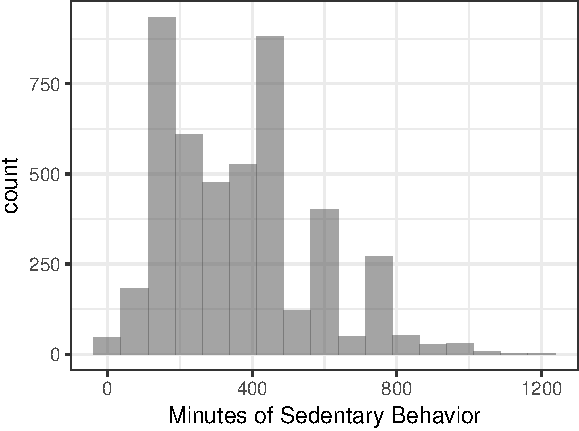
\includegraphics{05_GeneralizedLinearModels_files/figure-beamer/unnamed-chunk-7-1.pdf}

\end{frame}

\begin{frame}{Running Poisson Regression}

\Large
and so other methods related to poisson may be necessary.

\begin{itemize}
\tightlist
\item
  See gamma, hurdle models, and negative binomial models next
\end{itemize}

\end{frame}

\begin{frame}{Gamma}

\Large

\begin{itemize}
\tightlist
\item
  very similar to poisson but does not require integers and can handle
  more dispersion.
\item
  the outcome must have values \(> 0\).
\end{itemize}

\end{frame}

\begin{frame}[fragile]{Gamma}

\small

\begin{Shaded}
\begin{Highlighting}[]
\NormalTok{## Adjust sed}
\NormalTok{df}\OperatorTok{$}\NormalTok{sed_gamma <-}\StringTok{ }\NormalTok{df}\OperatorTok{$}\NormalTok{sed }\OperatorTok{+}\StringTok{ }\NormalTok{.}\DecValTok{01}
\NormalTok{g_fit <-}\StringTok{ }\KeywordTok{glm}\NormalTok{(sed_gamma }\OperatorTok{~}\StringTok{ }\NormalTok{asthma }\OperatorTok{+}\StringTok{ }\NormalTok{race }\OperatorTok{+}\StringTok{ }\NormalTok{famsize,}
             \DataTypeTok{data =}\NormalTok{ df,}
             \DataTypeTok{family =} \StringTok{"Gamma"}\NormalTok{)}
\KeywordTok{summary}\NormalTok{(g_fit)}
\end{Highlighting}
\end{Shaded}

\end{frame}

\begin{frame}[fragile]{Gamma}

\small

\begin{verbatim}
## 
## Call:
## glm(formula = sed_gamma ~ asthma + race + famsize, family = "Gamma", 
##     data = df)
## 
## Deviance Residuals: 
##     Min       1Q   Median       3Q      Max  
## -4.3589  -0.4613  -0.0845   0.2926   1.6868  
## 
## Coefficients:
##                     Estimate Std. Error t value Pr(>|t|)    
## (Intercept)        3.567e-03  1.132e-04  31.515  < 2e-16 ***
## asthma            -1.604e-04  5.865e-05  -2.735  0.00626 ** 
## raceOtherHispanic -4.874e-04  1.309e-04  -3.723  0.00020 ***
## raceWhite         -1.090e-03  1.078e-04 -10.115  < 2e-16 ***
## raceBlack         -1.068e-03  1.102e-04  -9.697  < 2e-16 ***
## raceOther         -1.110e-03  1.145e-04  -9.695  < 2e-16 ***
## famsize            5.107e-05  1.552e-05   3.289  0.00101 ** 
## ---
## Signif. codes:  0 '***' 0.001 '**' 0.01 '*' 0.05 '.' 0.1 ' ' 1
## 
## (Dispersion parameter for Gamma family taken to be 0.2932604)
## 
##     Null deviance: 1664.8  on 4436  degrees of freedom
## Residual deviance: 1604.2  on 4430  degrees of freedom
##   (195 observations deleted due to missingness)
## AIC: 59154
## 
## Number of Fisher Scoring iterations: 5
\end{verbatim}

\Large

\end{frame}

\begin{frame}[fragile]{Two-Part or Hurdle Models}

\large

\begin{itemize}
\tightlist
\item
  Use the \texttt{pscl} package to run a hurdle model.
\item
  These models are built for situations where there is a count variable
  with many zeros (``zero-inflated'').
\item
  The hurdle model makes slightly different assumptions regarding the
  zeros than the pure negative binomial that we present next.
\item
  The hurdle consists of two models: one for whether the person had a
  zero or more (binomial) and if more than zero, how many (poisson).
\end{itemize}

To run a hurdle model, we are going to make a sedentary variable with
many more zeros to illustrate and then we will run a hurdle model.

\end{frame}

\begin{frame}[fragile]{Two-Part or Hurdle Models}

\small

\begin{Shaded}
\begin{Highlighting}[]
\NormalTok{## Zero inflated sedentary (don't worry too much about the specifics)}
\NormalTok{df}\OperatorTok{$}\NormalTok{sed_zero <-}\StringTok{ }\KeywordTok{ifelse}\NormalTok{(}\KeywordTok{sample}\NormalTok{(}\DecValTok{1}\OperatorTok{:}\DecValTok{100}\NormalTok{, }
                             \DataTypeTok{size =} \KeywordTok{length}\NormalTok{(df}\OperatorTok{$}\NormalTok{sed), }
                             \DataTypeTok{replace=}\OtherTok{TRUE}\NormalTok{) }\OperatorTok\StringTok{ }\KeywordTok{c}\NormalTok{(}\DecValTok{5}\NormalTok{,}\DecValTok{10}\NormalTok{,}\DecValTok{11}\NormalTok{,}\DecValTok{20}\OperatorTok{:}\DecValTok{25}\NormalTok{), }\DecValTok{0}\NormalTok{, }
\NormalTok{                      df}\OperatorTok{$}\NormalTok{sed)}
\NormalTok{## Hurdle model}
\KeywordTok{library}\NormalTok{(pscl)}
\NormalTok{h_fit =}\StringTok{ }\KeywordTok{hurdle}\NormalTok{(sed_zero }\OperatorTok{~}\StringTok{ }\NormalTok{asthma }\OperatorTok{+}\StringTok{ }\NormalTok{race }\OperatorTok{+}\StringTok{ }\NormalTok{famsize,}
               \DataTypeTok{data =}\NormalTok{ df)}
\KeywordTok{summary}\NormalTok{(h_fit)}
\end{Highlighting}
\end{Shaded}

\normalsize

\end{frame}

\begin{frame}[fragile]{Two-Part or Hurdle Models}

\tiny

\begin{verbatim}
## 
## Call:
## hurdle(formula = sed_zero ~ asthma + race + famsize, data = df)
## 
## Pearson residuals:
##     Min      1Q  Median      3Q     Max 
## -3.9248 -1.4783 -0.2191  1.2563 11.0364 
## 
## Count model coefficients (truncated poisson with log link):
##                     Estimate Std. Error z value Pr(>|z|)    
## (Intercept)        5.6727458  0.0036627 1548.80   <2e-16 ***
## asthma             0.0627030  0.0022628   27.71   <2e-16 ***
## raceOtherHispanic  0.1201634  0.0042592   28.21   <2e-16 ***
## raceWhite          0.3248979  0.0034416   94.40   <2e-16 ***
## raceBlack          0.3337217  0.0035384   94.31   <2e-16 ***
## raceOther          0.3359265  0.0037427   89.75   <2e-16 ***
## famsize           -0.0200684  0.0005781  -34.71   <2e-16 ***
## Zero hurdle model coefficients (binomial with logit link):
##                   Estimate Std. Error z value Pr(>|z|)    
## (Intercept)        2.84791    0.23592  12.072   <2e-16 ***
## asthma            -0.20907    0.13695  -1.527   0.1269    
## raceOtherHispanic -0.57535    0.25379  -2.267   0.0234 *  
## raceWhite         -0.48597    0.22052  -2.204   0.0275 *  
## raceBlack         -0.31269    0.22953  -1.362   0.1731    
## raceOther         -0.37082    0.24153  -1.535   0.1247    
## famsize           -0.05421    0.03545  -1.529   0.1262    
## ---
## Signif. codes:  0 '***' 0.001 '**' 0.01 '*' 0.05 '.' 0.1 ' ' 1 
## 
## Number of iterations in BFGS optimization: 12 
## Log-likelihood: -2.307e+05 on 14 Df
\end{verbatim}

\Large

\end{frame}

\begin{frame}{Hurdle Models}

\large

Notice that the output has two parts:

\begin{enumerate}
\def\labelenumi{\arabic{enumi}.}
\tightlist
\item
  ``Count model coefficients (truncated poisson with log link):'' and
\item
  ``Zero hurdle model coefficients (binomial with logit link):''.
\end{enumerate}

Together they tell us about the relationship between the predictors and
a count variable with many zeros.

\end{frame}

\begin{frame}[fragile]{Negative Binomial}

\large

\begin{itemize}
\tightlist
\item
  negative binomial is also for zero-inflated count variables.
\item
  It makes slightly different assumptions than the hurdle and doesn't
  use a two-part approach.
\item
  Use the \texttt{MASS} package and the \texttt{glm.nb()} function.
\end{itemize}

\small

\begin{Shaded}
\begin{Highlighting}[]
\KeywordTok{library}\NormalTok{(MASS)}
\NormalTok{fit_nb <-}\StringTok{ }\KeywordTok{glm.nb}\NormalTok{(sed_zero }\OperatorTok{~}\StringTok{ }\NormalTok{asthma }\OperatorTok{+}\StringTok{ }\NormalTok{race }\OperatorTok{+}\StringTok{ }\NormalTok{famsize,}
                 \DataTypeTok{data =}\NormalTok{ df)}
\KeywordTok{summary}\NormalTok{(fit_nb)}
\end{Highlighting}
\end{Shaded}

\end{frame}

\begin{frame}{Negative Binomial}

\small

\Large

Note that this model is not really appropriate because our data is
somewhat contrived.

\end{frame}

\section{Beta Regression}\label{beta-regression}

\begin{frame}{Beta Regression}

\large

\begin{itemize}
\tightlist
\item
  For outcomes that are bound between a lower and upper bound
\item
  For example, if we are looking at test scores that are bound between 0
  and 100.
\item
  It is a very flexible method and allows for some extra analysis
  regarding the variation.
\end{itemize}

\end{frame}

\begin{frame}[fragile]{Running Beta Regression}

\begin{itemize}
\tightlist
\item
  Use the \texttt{betareg} package.
\item
  But first, we are going to reach a little and create a ficticiously
  bound variable in the data set.
\end{itemize}

\begin{Shaded}
\begin{Highlighting}[]
\NormalTok{## Variable bound between 0 and 1}
\NormalTok{df}\OperatorTok{$}\NormalTok{beta_var <-}\StringTok{ }\KeywordTok{sample}\NormalTok{(}\KeywordTok{seq}\NormalTok{(.}\DecValTok{05}\NormalTok{, .}\DecValTok{99}\NormalTok{, }\DataTypeTok{by =}\NormalTok{ .}\DecValTok{01}\NormalTok{), }
                      \DataTypeTok{size =} \KeywordTok{length}\NormalTok{(df}\OperatorTok{$}\NormalTok{asthma),}
                      \DataTypeTok{replace =} \OtherTok{TRUE}\NormalTok{)}
\KeywordTok{library}\NormalTok{(betareg)}
\NormalTok{fit_beta <-}\StringTok{ }\KeywordTok{betareg}\NormalTok{(beta_var }\OperatorTok{~}\StringTok{ }\NormalTok{asthma }\OperatorTok{+}\StringTok{ }\NormalTok{race }\OperatorTok{+}\StringTok{ }\NormalTok{famsize,}
                    \DataTypeTok{data =}\NormalTok{ df)}
\KeywordTok{summary}\NormalTok{(fit_beta)}
\end{Highlighting}
\end{Shaded}

\end{frame}

\begin{frame}[fragile]{Running Beta Regression}

\tiny

\begin{verbatim}
## 
## Call:
## betareg(formula = beta_var ~ asthma + race + famsize, data = df)
## 
## Standardized weighted residuals 2:
##     Min      1Q  Median      3Q     Max 
## -2.0364 -0.6739 -0.0598  0.6311  2.9235 
## 
## Coefficients (mean model with logit link):
##                    Estimate Std. Error z value Pr(>|z|)   
## (Intercept)        0.195018   0.063399   3.076   0.0021 **
## asthma            -0.057137   0.043789  -1.305   0.1920   
## raceOtherHispanic -0.053873   0.072158  -0.747   0.4553   
## raceWhite         -0.025079   0.058871  -0.426   0.6701   
## raceBlack         -0.059966   0.061116  -0.981   0.3265   
## raceOther         -0.077520   0.065502  -1.183   0.2366   
## famsize           -0.009472   0.010843  -0.874   0.3824   
## 
## Phi coefficients (precision model with identity link):
##       Estimate Std. Error z value Pr(>|z|)    
## (phi)  2.45394    0.04465   54.95   <2e-16 ***
## ---
## Signif. codes:  0 '***' 0.001 '**' 0.01 '*' 0.05 '.' 0.1 ' ' 1 
## 
## Type of estimator: ML (maximum likelihood)
## Log-likelihood:  83.2 on 8 Df
## Pseudo R-squared: 0.00112
## Number of iterations: 15 (BFGS) + 1 (Fisher scoring)
\end{verbatim}

\Large

\end{frame}

\begin{frame}{Beta Regression}

\large

\begin{itemize}
\tightlist
\item
  The output provides coefficients and the ``Phi'' coefficients.
\item
  Both are important parts of using beta regression but we are not going
  to discuss it here.
\end{itemize}

\end{frame}

\section{Conclusions}\label{conclusions}

\begin{frame}{Conclusions}

\large

There are many resources available to learn more about each of these
GLM's.

As for now, we are going to move on to more complex modeling where there
are clustering or repeated measures in the data.

\end{frame}

\begin{frame}[fragile]{Conclusions}

\large

One of the great things about \texttt{R} is that most modeling is very
similar to the basic \texttt{lm()} function.

\begin{itemize}
\tightlist
\item
  In all of these GLM's the arguments are nearly all the same:

  \begin{itemize}
  \tightlist
  \item
    a formula,
  \item
    the data, and
  \item
    family of model.
  \end{itemize}
\item
  As you'll see for Multilevel and Other Models chapters, this does not
  change much.
\item
  Having a good start with basic models and GLM's gets you ready for
  nearly every other modeling type in \texttt{R}.
\end{itemize}

\end{frame}
